\section{Introduction}
We consider a variant of the classic Art Gallery problem, where we instead seek to optimize the length of the boundary seen by the guards, not the number of guards themselves. Specifically, given a simple polygon $P$ and $k\in\mathbb{N}$, we want to find the $k$ vertex guards which maximize the length of the boundary of $P$ that is watched. We define the set of vertices of $P$ as $V_P$, and $L(S)$ as the length of the boundary seen by the set of vertex guards/vertices $S$. Note that $L(S)$ is necessarily at most the perimeter of $P$. 

\optproblemdef{\MLVG{}}{A simple polygon $P$ and a positive integer $k\in\mathbb{N}$.}{Find a set of vertices $S\subseteq V_P$ of size at most $k$ such that $L(S)$ is maximized.}

We also consider a weighted variant of this problem, where $P$ is a simple polygon composed of (possibly collinear) weighted line segments, such a polygon is depicted in~\Cref{fig:weighted-polygon}. Art galleries contain paintings, and some have more value than others. With limited guards, a realistic task would be to maximize not the total boundary watched, but the total value of paintings watched. In our problem, a weighted segment must be \emph{completely} seen by our $k$ guards to be considered ``guarded''. We define $W(S)$ as the weighted analog of $L(S)$, the sum of weights of all segments on the boundary of $P$ that are completely watched by guards in $S$.

\begin{figure}
    \centering
    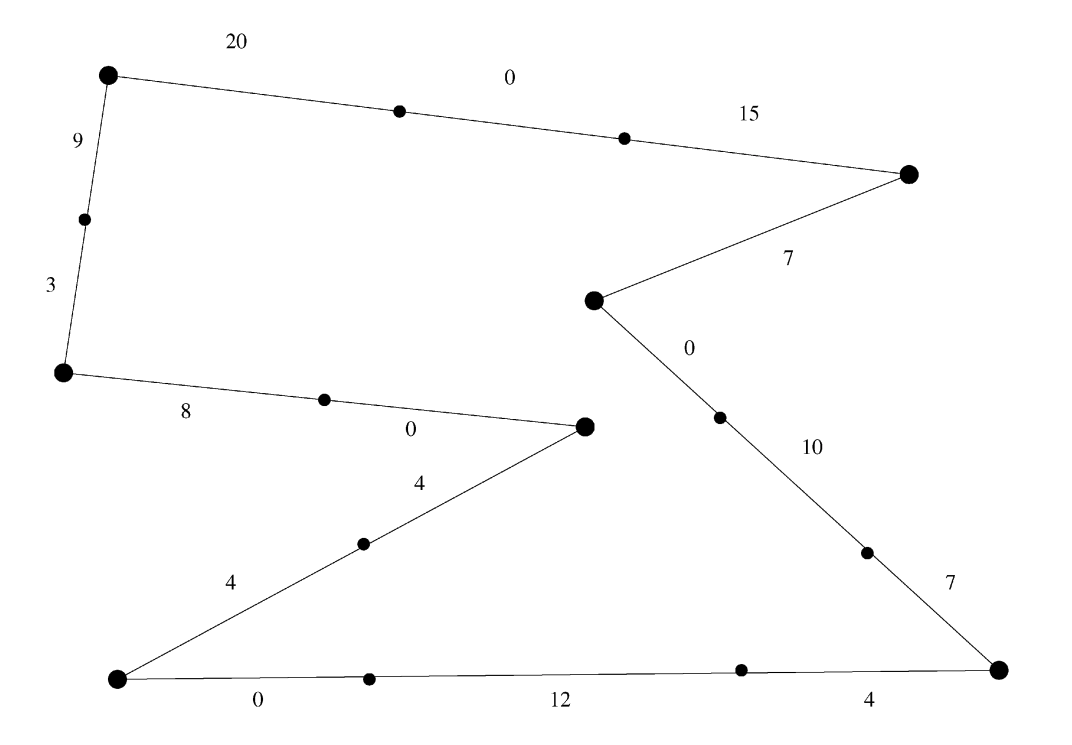
\includegraphics[width=8cm]{figures/weighted-polygon.png}
    \caption{A polygon composed of weighted line segments, the input for \MVVG{}.}
    \label{fig:weighted-polygon}
\end{figure}

\optproblemdef{\MVVG{}}{A weighted polygon $P$ and a positive integer $k\in\mathbb{N}$.}{Find a set of vertices $S\subseteq V_P$ of size at most $k$ such that $W(S)$ is maximized.}

We also introduce a version of \MVVG{} with cost, not cardinality constraints. It can be more expensive to place guards or cameras in certain parts of an art gallery --- we should not expect it to be equally viable to place a guard at any vertex in the polygon. Instead of being limited to $k$ vertex guards, we are given a budget $B$. Each vertex has a cost $c(v)\leq B$, and we must find the set of guards which maximizes the total weight guarded, such that the total cost of the set of guards is less than or equal to $B$.

\optproblemdef{\BMVVG{}}{A weighted polygon $P$ and a positive integer $B\in\mathbb{N}$.}{Find a set of vertices $S\subseteq V_P$ with $\sum_{s\in S}c(s)\leq B$ such that $W(S)$ is maximized.}

\subsection{Related Works}
\todo[inline]{Need a paragraph discussing more conventional Art gallery problem literature (authors+results). Klee, O'Rourke, Das}
In \cite{fragoudakis-interior,fragoudakis-boundary,fragoudakis-paintings}, Fragoudakis et al. pose both \MLVG\ and \MVVG. They prove that both problems are APX-complete in \cite{fragoudakis-boundary}, meaning these problems are NP-hard and also permit no PTAS unless $P=NP$. In \cite{fragoudakis-interior}, they present a $(1-1/e)$-approximation for maximizing the vertex-guarded \emph{interior} of a polygon which runs in $O(k^2n^2)$ and depends on segmenting the polygon into visibility regions.

\cite{abdelkader} presents several inapproximability results for art gallery problems, with $\alpha$-Floodlights.

\todo[inline]{Need to discuss some more dynamic set cover. Here is the most recent paper I've been able to find.}

\cite{bukov}

\subsection{Our Contributions}

For \MLVG{} and \MVVG{}, we improve upon the $(1-1/e)$-approximation with $O(k^2n^2)$ running time from \cite{fragoudakis-interior,fragoudakis-boundary,fragoudakis-paintings} by showing monotonoicty and submodularity of the objective function of each problem. This gives us a $(1-1/e)$-approximation which runs in $O(kn^2)$ time. We also show that this is the best possible approximation factor for these problems, which agrees well with their results of showing these problems are APX-complete.\\\\
We also propose a budgeted version of \MVVG{} that uses vertex costs instead of cardinality constraints, and then provide several examples demonstrating that three naive greedy strategies all fail to form approximations. These greedy strategies are (1) greedily choosing the vertex which maximizes the marginal gain in total weight guarded (2) greedily choosing the cheapest vertex and (3) greedily choosing the vertex which maximizes the ratio of marginal gain in total weight guarded to vertex cost. Equipped with these examples, we propose an idea based on \cite{khuller}, which might provide a $(1-1/e)$-approximation for \BMVVG{}. 

